\documentclass{beamer}\usepackage[]{graphicx}\usepackage[]{color}
%% maxwidth is the original width if it is less than linewidth
%% otherwise use linewidth (to make sure the graphics do not exceed the margin)
\makeatletter
\def\maxwidth{ %
  \ifdim\Gin@nat@width>\linewidth
    \linewidth
  \else
    \Gin@nat@width
  \fi
}
\makeatother

\definecolor{fgcolor}{rgb}{0.345, 0.345, 0.345}
\newcommand{\hlnum}[1]{\textcolor[rgb]{0.686,0.059,0.569}{#1}}%
\newcommand{\hlstr}[1]{\textcolor[rgb]{0.192,0.494,0.8}{#1}}%
\newcommand{\hlcom}[1]{\textcolor[rgb]{0.678,0.584,0.686}{\textit{#1}}}%
\newcommand{\hlopt}[1]{\textcolor[rgb]{0,0,0}{#1}}%
\newcommand{\hlstd}[1]{\textcolor[rgb]{0.345,0.345,0.345}{#1}}%
\newcommand{\hlkwa}[1]{\textcolor[rgb]{0.161,0.373,0.58}{\textbf{#1}}}%
\newcommand{\hlkwb}[1]{\textcolor[rgb]{0.69,0.353,0.396}{#1}}%
\newcommand{\hlkwc}[1]{\textcolor[rgb]{0.333,0.667,0.333}{#1}}%
\newcommand{\hlkwd}[1]{\textcolor[rgb]{0.737,0.353,0.396}{\textbf{#1}}}%

\usepackage{framed}
\makeatletter
\newenvironment{kframe}{%
 \def\at@end@of@kframe{}%
 \ifinner\ifhmode%
  \def\at@end@of@kframe{\end{minipage}}%
  \begin{minipage}{\columnwidth}%
 \fi\fi%
 \def\FrameCommand##1{\hskip\@totalleftmargin \hskip-\fboxsep
 \colorbox{shadecolor}{##1}\hskip-\fboxsep
     % There is no \\@totalrightmargin, so:
     \hskip-\linewidth \hskip-\@totalleftmargin \hskip\columnwidth}%
 \MakeFramed {\advance\hsize-\width
   \@totalleftmargin\z@ \linewidth\hsize
   \@setminipage}}%
 {\par\unskip\endMakeFramed%
 \at@end@of@kframe}
\makeatother

\definecolor{shadecolor}{rgb}{.97, .97, .97}
\definecolor{messagecolor}{rgb}{0, 0, 0}
\definecolor{warningcolor}{rgb}{1, 0, 1}
\definecolor{errorcolor}{rgb}{1, 0, 0}
\newenvironment{knitrout}{}{} % an empty environment to be redefined in TeX

\usepackage{alltt}
\usepackage[utf8]{inputenc}



\usepackage{url}
\ifx\hypersetup\undefined
  \AtBeginDocument{%
    \hypersetup{unicode=true,pdfusetitle,
 bookmarks=true,bookmarksnumbered=false,bookmarksopen=false,
 breaklinks=false,pdfborder={0 0 0},backref=false,colorlinks=false}
  }
\else
  \hypersetup{unicode=true,pdfusetitle,
 bookmarks=true,bookmarksnumbered=false,bookmarksopen=false,
 breaklinks=false,pdfborder={0 0 0},backref=false,colorlinks=false}
\fi

% Beamer style
%\usetheme[secheader]{Madrid}
\usetheme{CambridgeUS}
\usecolortheme[rgb={0.65,0.15,0.25}]{structure}
%\usefonttheme[onlymath]{serif}
\beamertemplatenavigationsymbolsempty


% Packages
\usepackage{dsfont, stmaryrd}
\usepackage{amsmath, amsfonts, amssymb}
\usepackage{rotating}
\usepackage{epsfig}
\usepackage{astats}
%\usepackage[all]{xy}
\usepackage{graphicx}
\usepackage{algorithm2e}

% Commands
\definecolor{darkgreen}{cmyk}{0.5, 0, 0.5, 0.5}
\definecolor{greenB}{rgb}{0.3, 0.87, 0.}
\definecolor{darkred}{rgb}{0.65,0.15,0.25}
\definecolor{darkblue}{rgb}{0.08,0.11,0.81}
\definecolor{lightblue}{rgb}{0.4,0.51,0.8}
\definecolor{darkorange}{rgb}{1,0.54,0}
\newcommand{\blue}[1]{\textcolor{blue}{#1}}
\newcommand{\hid}[1]{\textcolor{darkblue}{#1}}
\newcommand{\Ehid}[1]{\textcolor{lightblue}{#1}}
\newcommand{\obsy}[1]{\textcolor{red}{#1}}
\newcommand{\Eobsy}[1]{\textcolor{darkorange}{#1}}
\newcommand{\emphase}[1]{\textcolor{darkred}{#1}}
\newcommand{\emphaseBis}[1]{\textcolor{darkblue}{#1}}
\newcommand{\paragraph}[1]{\emphase{#1}}
\newcommand{\refer}[1]{\textcolor{blue}{\sl \cite{#1}}}
\newcommand{\Refer}[1]{\textcolor{blue}{\sl #1}}


%thm prop and co
\newtheorem{prop}{Proposition}

% Symbols
\def\d{\text{ d}} % Element differentiel
\newcommand{\Abf}{{\bf A}}
\newcommand{\Beta}{\text{B}}
\newcommand{\betabf}{\mbox{\mathversion{bold}{$\beta$}}}
\newcommand{\Bcal}{\mathcal{B}}
\newcommand{\BIC}{\text{BIC}}
\newcommand{\dd}{\text{d}}
\newcommand{\Cbf}{{\bf C}}
\newcommand{\dbf}{{\bf d}}
\newcommand{\Dcal}{\mathcal{D}}
\newcommand{\Esp}{\mathbb{E}}
\renewcommand{\P}{\mathbb{P}}
\newcommand{\Ebf}{{\bf E}}
\newcommand{\Ecal}{\mathcal{E}}
\newcommand{\Gcal}{\mathcal{G}}
\newcommand{\Gam}{\mathcal{G}\mbox{am}}
\newcommand{\Ibb}{\mathbb{I}}
\newcommand{\Ibf}{{\bf I}}
\newcommand{\ICL}{\text{ICL}}
\newcommand{\Cov}{\mathbb{C}\text{ov}}
\newcommand{\Corr}{\mathbb{C}\text{orr}}
\newcommand{\Var}{\mathbb{V}}
\newcommand{\Vsf}{\mathsf{V}}
\newcommand{\pen}{\text{pen}}
\newcommand{\Fcal}{\mathcal{F}}
\newcommand{\Hbf}{{\bf H}}
\newcommand{\Hcal}{\mathcal{H}}
\newcommand{\Jcal}{\mathcal{J}}
\newcommand{\Kbf}{{\bf K}}
\newcommand{\Lcal}{\mathcal{L}}
\newcommand{\Mcal}{\mathcal{M}}
\newcommand{\mbf}{{\bf m}}
\newcommand{\mum}{\mu(\mbf)}
\newcommand{\Ncal}{\mathcal{N}}
\newcommand{\Nbf}{{\bf N}}
\newcommand{\Nm}{N(\mbf)}
\newcommand{\Ocal}{\mathcal{O}}
\newcommand{\Obf}{{\bf 0}}
\newcommand{\Omegas}{\underset{s}{\Omega}}
\newcommand{\Pbf}{{\bf P}}
\newcommand{\Pcal}{\mathcal{P}}
\newcommand{\Qcal}{\mathcal{Q}}
\newcommand{\Rbb}{\mathbb{R}}
\newcommand{\Rbf}{{\bf R}}
\newcommand{\Rcal}{\mathcal{R}}
\newcommand{\sbf}{{\bf s}}
\newcommand{\Sbf}{{\bf S}}
\newcommand{\Scal}{\mathcal{S}}
\newcommand{\Ucal}{\mathcal{U}}
\newcommand{\Vcal}{\mathcal{V}}
\newcommand{\Tbf}{{\bf T}}
\newcommand{\ubf}{{\bf u}}
\newcommand{\Ubf}{{\bf U}}
\newcommand{\Wbf}{{\bf W}}
\newcommand{\xbf}{{\bf x}}
\newcommand{\Xbf}{{\bf X}}  
\newcommand{\Ybf}{{\bf Y}}
\newcommand{\Zbf}{{\bf Z}}
\newcommand{\pibf}{\mbox{\mathversion{bold}{$\pi$}}}
\newcommand{\Pibf}{\mbox{\mathversion{bold}{$\Pi$}}}
\newcommand{\Sigmabf}{\mbox{\mathversion{bold}{$\Sigma$}}}
\newcommand{\gammabf}{\mbox{\mathversion{bold}{$\gamma$}}}
  \newcommand{\mubf}{\mbox{\mathversion{bold}{$\mu$}}}
\newcommand{\nubf}{\mbox{\mathversion{bold}{$\nu$}}}
\newcommand{\Thetabf}{\mbox{\boldsymbol{\Theta}}}
\newcommand{\thetabf}{\mbox{\mathversion{bold}{$\theta$}}}
\newcommand{\BP}{\text{BP}}
\newcommand{\EM}{\text{EM}}
\newcommand{\VEM}{\text{VEM}}
\newcommand{\VBEM}{\text{VB}}
\newcommand{\cst}{\text{cst}}
\newcommand{\obs}{\text{obs}}
\newcommand{\ra}{\emphase{\mathversion{bold}{$\rightarrow$}~}}
\newcommand{\QZ}{Q_{\Zbf}}
\newcommand{\Qt}{Q_{\thetabf}}
\def\argmax{\mathop{\mathrm{argmax}}}


% Directory
\newcommand{\FigSim}{}
%{/RECHERCHE/RUPTURES/MinRegionCont/Res}
\graphicspath{{figure/}{..//figure/}}
%--------------------------------------------------------------------

\title{Model based detection of homogeneous portions in trajectories}

\author[MP Etienne]{Marie-Pierre Etienne }

 \institute[AgroParisTech / INRA]{  AgroParisTech / INRA \\
   \bigskip
   \begin{tabular}{cccc}
    
\includegraphics[ height=1cm]{logagrotech_ABL_RVB}& 
    \hspace{.5cm} &
     \includegraphics[height=1cm]{logotype-INRA-RVB} & 
   \end{tabular} \\ 
   \bigskip
   }

\date[Movement Ecology]{Movement Ecology Workshop 2015 - Port Elizabeth}

%--------------------------------------------------------------------

%--------------------------------------------------------------------
%--------------------------------------------------------------------
\IfFileExists{upquote.sty}{\usepackage{upquote}}{}
\begin{document}



%--------------------------------------------------------------------
%--------------------------------------------------------------------

%--------------------------------------------------------------------
 \frame{\titlepage
   }
% %--------------------------------------------------------------------
% %--------------------------------------------------------------------
\frame{
\tableofcontents[subsectionstyle=hide]  }


% %--------------------------------------------------------------------
% %--------------------------------------------------------------------
\section{Introduction and Notations}


\subsection*{Motivation}
\begin{frame}[fragile]{Detection of homogenous regions in trajectories}

  \paragraph{Why ?}
\begin{columns}
\begin{column}{0.4\textwidth}
\begin{itemize}
\item Different behaviours.
\item Link with different activities.
\item Link with different environmental conditions.
\end{itemize}

\end{column}
\begin{column}{0.6\textwidth}



  
  \only<1>{\includegraphics[scale=0.4]{pathPractical2-1.pdf}}
\only<2>{\includegraphics[scale=0.4]{pathPractical3-1.pdf}}
\end{column}
\end{columns}
\end{frame}



\subsection*{Trajectories, a certain aspect of the movement}
\begin{frame}[fragile]{Effect of sampling step}

  \only<1>{\includegraphics[scale=0.4]{pathPractical4-1.pdf}}
\only<2>{\includegraphics[scale=0.4]{pathPractical4-3.pdf}}
\only<3>{\includegraphics[scale=0.4]{pathPractical4-6.pdf}}
\only<4>{\includegraphics[scale=0.4]{pathPractical4-10.pdf}}
\only<5>{\includegraphics[scale=0.4]{pathPractical4-15.pdf}}

  \only<6>{\includegraphics[scale=0.4]{pathPractical5-1.pdf}} 
\end{frame}


\begin{frame}{Summarising trajectories}
$(t_1, \ldots, t_N)$ denotes the time acquisition and $( (x_1,y_1),  \ldots, (x_N,y_N))$ the position at those times.

\only<1>{
  \paragraph{Trajetories as Turning angle and Speed}
  \begin{columns}
  \begin{column}{0.4\textwidth}
  
  $$\boldsymbol{\Phi}=(\phi_{2}, \ldots,\phi_{N})$$
    $$\boldsymbol{S}=(S_{2}, \ldots,\S_{N}),$$
    with $S_i=dist_i/(t_i-t_{i-1})$
    \end{column}
  \begin{column}{0.6\textwidth}
  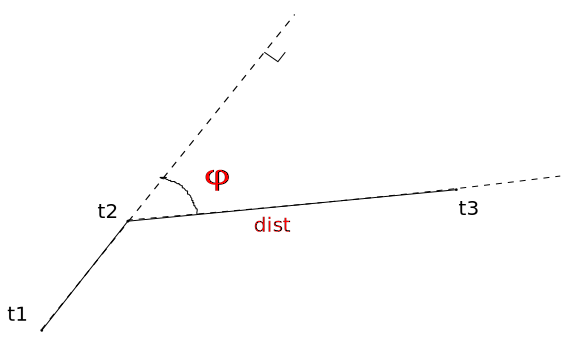
\includegraphics[scale=0.3]{Speed1.pdf}
  \end{column}
  \end{columns}
  $$ $$
}
\only<2>{
  \paragraph{Trajetories as Persistent and Normal Velocity}
  \begin{columns}
  \begin{column}{0.4\textwidth}
  
  $$\boldsymbol{V}^P=(V^P_{2}, \ldots,V^P_{N})$$
    $$\boldsymbol{V}^N=(V^N_{2}, \ldots,V^N_{N})$$
    with 
  \begin{align*}
  V^P_i&=S_i \, cos(\phi_i)\\
  V^N_i&=S_i \, sin(\phi_i)
  \end{align*}
  \end{column}
  \begin{column}{0.6\textwidth}
  \includegraphics[scale=0.3]{Speed2.pdf}
  \end{column}
  \end{columns}
}
\end{frame}


\begin{frame}{From Trajectories data to signal - Loosing information on spatial location}
\paragraph{How trajectories data migh be considered?}
\begin{itemize}
\item A sequence of (time, position)
\item Turning angle and speed sequences
\item Persistent and Normal Velocity sequences
\end{itemize}
\pause
\paragraph{What is affected by sampling?}
\begin{itemize}
\item A sequence of (time, position)
\item Turning angle and speed sequences
\item Persistent and Normal Velocity sequences
\end{itemize}
\pause
\paragraph{Model approach:}
\begin{itemize}
\item Most methods don't consider the two phenomena : movement and sampling process.
  \item Results will be closely dependent of the sampling step.
  \end{itemize}
\end{frame}

\subsection*{Statistical concepts}
\begin{frame}{Model and parameters}
\paragraph{The model} is a tentative to represent the main characteristics of potential data. \\

\only<2>{
If we observe the size of people $Y$ and assume $Y\sim\Ncal(\mu, \sigma)$
\includegraphics[scale=0.3]{Normal1.pdf}}
\only<3>{
If  people are sampled at random (with no relationship)
$$Y_i\overset{\blue{i.i.d}}{\sim}\Ncal(\mu, \sigma)$$
}
\onslide<4->{
$$Y_i\overset{\blue{i.i.d}}{\sim}\Ncal(\mu, \sigma)$$
\paragraph{The parameters} rule the behaviour of the model.\\
\only<4>{\includegraphics[scale=0.2]{Normal2.pdf}}
\only<5>{\includegraphics[scale=0.2]{Normal3.pdf}}
}
\end{frame}

\begin{frame}{Estimation}
\paragraph{Simulation context:} with a given model $M$, and given parameters $\thetabf$, you can produce fake data. \\
From ($M, \thetabf$) to $\Ybf$.
\pause

\paragraph{Estimation context:} with a given model $M$, and some data $\Ybf$, you want to determine a good value for $\thetabf$. \\
From ($M, \Ybf$) to $\thetabf$.

\pause
\paragraph{What is a good value for $\thetabf$?} with a given model $M$, and some data $\Ybf$, you want to give a score to each possible value of $\thetabf$. 
\pause

\paragraph{The likelihood as a measure of the quality of $\thetabf$:} with a given model $M$, and some data $\Ybf$, for each value of $\thetabf$ you can compute the probability 
$$\P(\Ybf; \thetabf)$$

\end{frame}


\begin{frame}{Statistics and Hidden variables}
A model ($M, \thetabf$) produce $\Ybf$ and $\Zbf$.
\pause

The only observed data are $\Ybf$ while  $\Zbf$ are hidden variables.
\pause


Questions are 
\begin{itemize}
\item \blue{Parameters:} Is it still possible to estimate $\thetabf$ ?
\item \blue{Information on $\Zbf$:} is it possible to "reconstruct" the unobserved data $\Zbf$ ?
\end{itemize}

\pause

Bayes formula is the key :

$$\P(\Ybf, \Zbf)=\P(\Ybf \vert \Zbf)\P(\Zbf)=\P(\Zbf\vert \Ybf) \P(\Ybf)$$

\end{frame}



\subsection*{Convention}


\begin{frame}{Convention}
\paragraph{Notations:}
{\small
\begin{itemize}
\item $\Ybf = (Y_1, \ldots, Y_n) = $ observed data (typically Speed)
 \item $\Zbf= (Z_1, \ldots, Z_n) $ unobserved data (typically State, for mixture  and Hidden Markov model)
 \item \thetabf = the unknown parameters of $\Ybf$ and $\Zbf$.
\end{itemize}
}
\pause
\paragraph{Graphical Representation (DAG):}  \medskip
\begin{columns}
\begin{column}{0.3\textwidth}
\centering{Change point}\\ \smallskip
\includegraphics[scale=0.4]{Dag1.pdf}
\end{column}
\pause


\begin{column}{0.3\textwidth}
\centering{Mixture}\\ \smallskip
\includegraphics[scale=0.4]{Dag2.pdf}
\end{column}
\pause
\begin{column}{0.3\textwidth}
\centering{HMM}\\ \smallskip
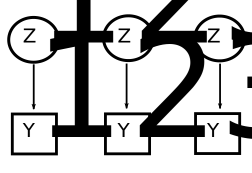
\includegraphics[scale=0.4]{Dag3.pdf}
\end{column}
\end{columns}
\end{frame}

%#show plan at the beginning of each secion except the first one
\AtBeginSection[]
{
 \begin{frame}<beamer>
 \frametitle{Plan}
 \tableofcontents[currentsection]
 \end{frame}
}

% %--------------------------------------------------------------------
% %--------------------------------------------------------------------
\section{Change point model}

\subsection*{Goal}
  \frame{\frametitle{Change point detection context}
    \begin{tabular}{p{0.4\textwidth} p{0.4\textwidth}}
    \begin{tabular}{p{\textwidth}}
        \includegraphics<1>[height=.6\textheight]{rawSignal}
        \includegraphics<2>[height=.6\textheight]{segmentedSignal}
      \end{tabular}
    &  
      \begin{tabular}{p{0.55\textwidth}}
        \onslide<1>{ \blue{Goal: } Identifying homogenous regions and abrupt changes in the signal.\\}
        \onslide<2>{ These \textcolor{red}{regions} may be interpreted afterwards.\\}
    \end{tabular}
  \end{tabular}
  }


\subsection*{Model}
\begin{frame}{Underlying model}


\only<1>{ Modelling~:}
\only<2>{\textcolor{red}{Change point detection in the trend (and/or in variance)~:} }
    \begin{itemize}
    \item Data $Y_1,\ldots,Y_n$ are drawn from a given pdf, driven by unknown parameter $\theta$
      \begin{equation*}
        Y_i \overset{i.i.d}{\sim} f_{\theta}(.)  \ \ 
      \end{equation*}
     $\theta$ values change at  $K-1$ unknow instants, the change point~:
     $t_1,\ldots,t_{K-1}$ :
     \only<1>{\begin{equation*}
         Y_t \sim f(\theta_k) \ \ \mbox{if $t$ in region $I_k=[t_{k-1}+1,t_{k}]$}
        \end{equation*}}
       \only<2->{ \textcolor{red}{
           \begin{equation*}
             Y_t\overset{ind}{\sim} \Ncal(\mu_k,\sigma^2) 
             \mbox{ if $t$ in portion $I_k$,  for  $k=1,\ldots,K$. }
           \end{equation*}
       } }
       \end{itemize}

  

 \onslide<3->{
  \begin{columns}
  \begin{column}{0.7\textwidth}
   \includegraphics[scale=0.3]{segCode1-1.pdf}
   \end{column}
   \begin{column}{0.3\textwidth}
  \noindent Remark : $K-1$ change points  $\Leftrightarrow$ $K$ regions.
   \end{column}
   \end{columns}
  }
\end{frame}

 
 \subsection*{Estimation}
 \frame{\frametitle{Estimation procedure}
   \begin{itemize}
   \item Unknown parameters : $\mubf=(\mu_1, \ldots, \mu_{\textcolor{red}{K}})$, $\sigma$, and $\Tbf=(T_1, \ldots, T_{\textcolor{red}{K}})$,\\
     but  also \textcolor{red}{K} itself.
   \onslide<3->{
   \item Estimation Procedure
   \only<3->{
    \begin{itemize}}
    \only<3>{
       \item For  given $K$ and $\Tbf$,   $\thetabf$ is estimated using maximum likelihood.}
       \only<4>{\item For  given $K$, compute the maximum likelihood for any possible position for $\Tbf$, 
       \textcolor{red}{But, } $$\left( \begin{array}{c} n-1 \\ K-1 \end{array}\right)$$ possible choices for the $K-1$ positions, that is $10^{30}$ for $K=10$, $n=200$,  ( $\approx 10^{11}$ years on a 2014 computer).
       \pause
  \centerline{$\Rightarrow$ Practically impossible even for small $K$ and $n$}
  \centerline{\textcolor{red}{Dynamic programming}}
       }
  \only<5>{
  \item Estimating $K$. 
     Likelihood increases with the number of segment $K$, use a penalized likelihood criterion and
    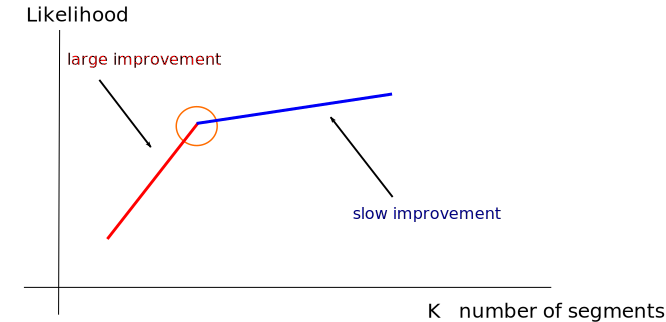
\includegraphics[scale=0.3]{LikelihoodProfile}
  }
  \only<3->{\end{itemize}}
   }
\end{itemize} 
}


\frame{\frametitle{Estimation procedure}

\paragraph{Likelihood}
{\small
\begin{eqnarray*}
2 log(P_K (\Ybf, \Tbf, \thetabf)) & = & 2 \sum_{k=1}^K \log f(\{Y_t\}_{t \in
I_k};
\theta_k) = 2 \sum_{k=1}^K \sum_{t \in I_k}\log f(Y_t; \theta_k) \\
& = & -n \log \sigma^2 - \frac1{\sigma^2} \sum_{k=1}^K \sum_{t \in
  I_k} (Y_t - \mu_k)^2 + \mbox{cst}.
\end{eqnarray*}
}

\paragraph{Estimations}
\begin{equation*}
 (\hat{\Tbf},\hat{\thetabf})=
  \argmax_{(\Tbf,\thetabf)} log(P_K (\Ybf, \Tbf, \thetabf))
\end{equation*}

\paragraph{If the change points are known}
\begin{columns}
\begin{column}{0.5\textwidth}
\begin{equation*}
\widehat{\mu}_k = \frac1{n_k} \sum_{t \in I_k} Y_t
\end{equation*}
\end{column}
\begin{column}{0.5\textwidth}
  $$
  \widehat{\sigma}^2 =  \frac1{n} \sum_{k=1}^K \sum_{t \in I_k} (Y_t -  \widehat{\mu}_k)^2
  $$
\end{column}
\end{columns}
}
% 
\begin{frame}[fragile]{Finding the K-1 change points}
 \only<1-3>{
 \paragraph{Considering all possible segmentations, } the best segmentation minimizes 
 $$
 J_k(1, n) = \sum_{k=1}^K \sum_{t \in I_k} (Y_t - \widehat{\mu}_k)^2.
 $$
 \pause
 \paragraph{Dynamic programming,} with complexity ($\mathcal{O}(n^2)$).
 } 
 
% %possible only because the quantity of interest is the sum over all segments 
% 
% %%%%%%%%%%%%%%%%%%%%%%%%%%%%%%%%%%%%%%%%%%%%%%%%%%%%%%%%%%%%%%%%%%%%%%
% %%%%%%%%%%%%%%%%%%%%%%%%%%%%%%%%%%%%%%%%%%%%%%%%%%%%%%%%%%%%%%%%%%%%%%
 \only<4>{\centerline{\sl Sub-paths of the optimal path are themselves
 optimal,} 
 Bellmann optimality 
 $$ $$
 \begin{description}
% 
 \item[Initialisation:] Compute for $0 \leq i < j \leq n$, cost of portion $I_{ij}$~:
  $$
  J_1(i, j) = \sum_{t=i+1}^j (Y_t - \widehat{\mu})^2
  $$
 \item[Etape $k$:] Compute for $2 \leq k \leq K$, $J_k(i, j)$ the cost of the best segmentation in $k$ segments between $i$ and $j$.
   $$
   J_k(i, j) = \min_{i < h <j} \left[J_{k-1}(i, h) + J_1(h+1,  j)\right].
   $$
 \end{description}
 }
\end{frame}

% 
\subsection*{Example}
\subsection*{ Toy Example}
   \begin{frame}[fragile]{How to perform this segmentation approach ?}
 
\begin{columns}
\begin{column}{0.4\textwidth}
\begin{knitrout}\tiny
\definecolor{shadecolor}{rgb}{0.969, 0.969, 0.969}\color{fgcolor}\begin{kframe}
\begin{alltt}
\hlkwd{load}\hlstd{(}\hlstr{"../Data/dataSegmentation.Rd"}\hlstd{)}
\hlkwd{summary}\hlstd{(Profil.seg)}
\end{alltt}
\begin{verbatim}
   Min. 1st Qu. 
 0.8904  4.8720 
 Median    Mean 
 5.6990  5.3660 
3rd Qu.    Max. 
 6.3070  8.9400 
\end{verbatim}
\begin{alltt}
\hlkwd{plot}\hlstd{(Profil.seg)}
\end{alltt}
\end{kframe}
\end{knitrout}
\end{column}
\begin{column}{0.5\textwidth}
\includegraphics[scale=0.35]{segCode2-1.pdf}
\end{column}
\end{columns}
\end{frame}

\subsection*{Practical Example}
   \begin{frame}[fragile]{How to perform this segmentation approach ?}
\begin{columns}
\begin{column}{0.4\textwidth}
\begin{knitrout}\tiny
\definecolor{shadecolor}{rgb}{0.969, 0.969, 0.969}\color{fgcolor}\begin{kframe}
\begin{alltt}
\hlkwd{library}\hlstd{(}\hlstr{'cghseg'}\hlstd{)}
\hlcom{## format data into CGHdata}
\hlstd{signalCGH}    \hlkwb{<-} \hlkwd{new}\hlstd{(}\hlstr{"CGHdata"}\hlstd{,}\hlkwc{Y}\hlstd{=Profil.seg)}
\hlstd{CGHo}         \hlkwb{<-} \hlkwd{new}\hlstd{(}\hlstr{"CGHoptions"}\hlstd{)}
\hlkwd{calling}\hlstd{(CGHo)}\hlkwb{<-} \hlnum{FALSE} \hlcom{## no classification }
\hlstd{segSignal}   \hlkwb{<-} \hlkwd{uniseg}\hlstd{(}\hlkwc{.Object}\hlstd{=signalCGH,}\hlkwc{CGHo}\hlstd{=CGHo)}
\hlstd{segSignalProf} \hlkwb{<-} \hlkwd{getsegprofiles}\hlstd{(segSignal)}
\hlkwd{plot}\hlstd{(Profil.seg)}
\hlkwd{lines}\hlstd{(}\hlnum{1}\hlopt{:}\hlkwd{length}\hlstd{(segSignalProf),}
      \hlstd{segSignalProf,} \hlkwc{type}\hlstd{=}\hlstr{"s"}\hlstd{,} \hlkwc{col}\hlstd{=}\hlnum{2}\hlstd{,} \hlkwc{lwd}\hlstd{=}\hlnum{2}\hlstd{)}
\end{alltt}
\end{kframe}
\end{knitrout}
\end{column}
\begin{column}{0.5\textwidth}
\includegraphics[scale=0.35]{segCode3-1.pdf}
\end{column}
\end{columns}
\end{frame}
% 

%  
 \begin{frame}[fragile]{Do it yourself}

\begin{columns}
\begin{column}{0.4\textwidth}
\begin{knitrout}\tiny
\definecolor{shadecolor}{rgb}{0.969, 0.969, 0.969}\color{fgcolor}\begin{kframe}
\begin{alltt}
\hlkwd{load}\hlstd{(}\hlkwc{file}\hlstd{=}\hlstr{"../Data/trajEx.Rd"}\hlstd{)}
\hlkwd{plot}\hlstd{(traj.ex,} \hlkwc{addpoints} \hlstd{= F)}
\hlkwd{legend}\hlstd{(}\hlstr{"bottomleft"}\hlstd{,}\hlkwc{pch}\hlstd{=}\hlkwd{c}\hlstd{(}\hlnum{2}\hlstd{,} \hlnum{0}\hlstd{),} \hlkwc{col}\hlstd{=}\hlkwd{c}\hlstd{(}\hlnum{4}\hlstd{,}\hlnum{2}\hlstd{),}
       \hlkwc{legend}\hlstd{=}\hlkwd{c}\hlstd{(}\hlstr{"Start"}\hlstd{,} \hlstr{"End"}\hlstd{),} \hlkwc{bty} \hlstd{=} \hlstr{"n"}\hlstd{,}
       \hlkwc{pt.lwd} \hlstd{=} \hlkwd{c}\hlstd{(}\hlnum{1.5}\hlstd{,}\hlnum{1.5}\hlstd{),} \hlkwc{pt.cex} \hlstd{=} \hlkwd{c}\hlstd{(}\hlnum{1.5}\hlstd{,}\hlnum{1.5}\hlstd{))}
\end{alltt}
\end{kframe}
\end{knitrout}
\end{column}
\begin{column}{0.5\textwidth}
\includegraphics[scale=0.35]{Practical1-1.pdf}
\end{column}
\end{columns}
\end{frame}

\subsection*{Clustering Segmentation}
%%%%%%%%%%%%%%%%%%%%%%%%%%%%%%%%%%%%%%%%%%%%%%%%%%%%%%%%%%
\begin{frame}{When Segmentation is not sufficient - clustering segmentation model}
$$
\begin{tabular}{cc}
  Pure segmentation & Segmentation + classification \\
  \includegraphics[scale=0.3]{FigSegClas-1.pdf} &
  \includegraphics[scale=0.3]{FigSegClas-2.pdf} 
  \end{tabular}
$$
\end{frame}



\begin{frame}{Segmentation-Clustering}
 \begin{itemize}
%  \item Assuming a \textcolor{blue}{secondary underlying
%      structure} of the segments into $P$ groups with weights
%    $\pi_1,...,\pi_P (\sum_p \pi_p=1)$.
%    \pause
%  \item Let's define \emphase{hidden variables $Z_{kp}$}, indicators of the
%    \emphase{group to which segment $k$ belongs}.
%    \pause
%  \item $\pi_p$ denotes the \emphase{proportion} of group $p$.
%  \pause
 \item The \emphase{distribution of the signal} given the group of the
     segment is
   \begin{align*}
    t \in I_k, k \in p &\qquad \Rightarrow \qquad Y_t \sim
    \Ncal(m_{\emphase{p}}, \sigma^2)\\
    Y^k|Z_{kp}=1 &\sim \Ncal( m_p, \sigma^2 ).
    \end{align*}
 \item It is a model of \blue{segmentation / clustering}.
 \pause
  \item \blue{Model parameters are $\thetabf =(\pibf, \gammabf)$} and 
  the breakpoint positions $\blue{\Tbf = (t_1, ..., t_{K-1})}$.
\end{itemize}
\end{frame} 
% 
% 
\begin{frame}{Hybrid algorithm}
\only<1>{
\paragraph{2 levels of statistical units} 
 \begin{itemize}
 \item  The inference of the \emphase{breakpoints $T$}
   is made at the \emphase{position level $t$};
 \item  The inference of the \emphase{groups (status)
     ($\gammabf, \tau_{kp}$)} is made at the \emphase{segment level $k$}.
 \end{itemize}
} 
\only<2>{
  \paragraph{Alternate parameters estimation with $K$ and $P$ known}
 \begin{enumerate}
 \item  When $\Tbf$ is fixed, the
   \textcolor{blue}{Expectation-Maximisation (EM)} algorithm estimates
   $\thetabf$;
   $$
    \hat{\thetabf}^{(h+1)}=\underset{\thetabf}{\arg\max} \left\{\log
      \Lcal_{KP}\left(\thetabf,T^{(h)}\right) \right\}. 
   $$
    $$
    \log \Lcal_{KP}( \hat{\thetabf}^{(h+1)}; \hat{\Tbf}^{(h)})
    \geq \log \Lcal_{KP}(\hat{\thetabf}^{(h)};
   \hat{\Tbf}^{(h)})
   $$
  \item  When $\thetabf$ is fixed, \textcolor{blue}{dynamic
      programming} estimates $\Tbf$;
     $$
    \hat{\Tbf}^{(h+1)}=\underset{\Tbf}{\argmax}
    \left\lbrace\log
      \Lcal_{KP}\left(\hat{\thetabf}^{(h+1)},\Tbf\right) \right\rbrace. 
   $$
   $$
   \log \Lcal_{KP}(\hat{\thetabf}^{(h+1)}; \hat{\Tbf}^{(h+1)})
   \geq \log \Lcal_{KP}(\hat{\thetabf}^{(h+1)};
   \hat{\Tbf}^{(h)})
   $$
    \end{enumerate} 
}
\end{frame}
%  

\subsection*{Example}
\subsection*{Toy Example}
   \begin{frame}[fragile]{How to perform this segmentation/clustering approach ?}
 
\begin{columns}
\begin{column}{0.4\textwidth}
\begin{knitrout}\tiny
\definecolor{shadecolor}{rgb}{0.969, 0.969, 0.969}\color{fgcolor}\begin{kframe}
\begin{alltt}
\hlcom{## format data into CGHdata}
\hlkwd{calling}\hlstd{(CGHo)}\hlkwb{<-} \hlnum{TRUE} \hlcom{## no classification }
\hlstd{CGHo}\hlopt{@}\hlkwc{nblevels}\hlkwb{=}\hlnum{2}
\hlstd{segSignal}   \hlkwb{<-} \hlkwd{uniseg}\hlstd{(}\hlkwc{.Object}\hlstd{=signalCGH,}\hlkwc{CGHo}\hlstd{=CGHo)}
\hlstd{segSignalProf} \hlkwb{<-} \hlkwd{getsegprofiles}\hlstd{(segSignal)}
\hlkwd{plot}\hlstd{(Profil.seg)}
\hlkwd{lines}\hlstd{(}\hlnum{1}\hlopt{:}\hlkwd{length}\hlstd{(segSignalProf),}
      \hlstd{segSignalProf,} \hlkwc{type}\hlstd{=}\hlstr{"s"}\hlstd{,} \hlkwc{col}\hlstd{=}\hlnum{2}\hlstd{,} \hlkwc{lwd}\hlstd{=}\hlnum{2}\hlstd{)}
\end{alltt}
\end{kframe}
\end{knitrout}
\end{column}
\begin{column}{0.5\textwidth}
\includegraphics[scale=0.35]{segCode4-1.pdf}
\end{column}
\end{columns}
\end{frame}

\subsection*{Practical Example}
\begin{frame}[fragile]{Do it yourself}
\end{frame}
% %--------------------------------------------------------------------
% %--------------------------------------------------------------------
% \section{Mixture Model}
% <<childMixture, child='Mixture.Rnw'>>=
% @
% %--------------------------------------------------------------------
% %--------------------------------------------------------------------
\section{Hidden Markov Model}

\subsection*{Model}
\begin{frame}{Markov chain model}
\paragraph{Modelling the dependence in state sequence:}
If an animal is feeding at time $i$, he has more chance to be feeding at time $i+1$ than if he was travelling at time $i$.
$$P(Z_{i+1}=1 \vert Z_{i}=1) \ne P(Z_{i+1}=1 \vert Z_{i}=2)$$

\paragraph{Markov Chain definition}
$\Zbf$ is a Markov chain if 
$$P(Z_{i+1} \vert Z_{1:i}) =  P(Z_{i+1} \vert Z_{i})$$


$\Zbf$ is completely defined by the distribution $\nu_1=P(Z_1)$ and the transition matrix
$$\Pi =\left[\begin{matrix}
\pi_{11} & 1-\pi_{11}\\
1-\pi_{22} & 1-\pi_{22}
\end{matrix}\right]$$
\end{frame}

\begin{frame}[fragile]{Markov chain simulation}

\begin{columns}
\begin{column}{0.5\textwidth}
\begin{knitrout}\tiny
\definecolor{shadecolor}{rgb}{0.969, 0.969, 0.969}\color{fgcolor}\begin{kframe}
\begin{alltt}
\hlcom{### Hidden State simulation}
\hlkwd{set.seed}\hlstd{(}\hlnum{6}\hlstd{)}
\hlstd{N} \hlkwb{<-} \hlnum{200}
\hlstd{pi11} \hlkwb{<-} \hlnum{0.8}
\hlstd{pi22} \hlkwb{<-} \hlnum{0.9}
\hlcom{## initial distribution}
\hlstd{mu1} \hlkwb{<-} \hlkwd{c}\hlstd{(}\hlnum{0.5}\hlstd{,} \hlnum{0.5}\hlstd{)}
\hlcom{##transition matrix}
\hlstd{PI} \hlkwb{<-} \hlkwd{matrix}\hlstd{(}\hlkwd{c}\hlstd{(pi11,} \hlnum{1}\hlopt{-}\hlstd{pi11,} \hlnum{1}\hlopt{-}\hlstd{pi22, pi22),} \hlkwc{ncol}\hlstd{=}\hlnum{2}\hlstd{,} \hlkwc{byrow} \hlstd{= T)}

\hlcom{##initialisation of Z}
\hlstd{Z} \hlkwb{<-} \hlkwd{rep}\hlstd{(}\hlnum{NA}\hlstd{, N)}
\hlstd{Z[}\hlnum{1}\hlstd{]} \hlkwb{<-} \hlkwd{sample}\hlstd{(}\hlnum{1}\hlopt{:}\hlnum{2}\hlstd{,} \hlkwc{size}\hlstd{=}\hlnum{1}\hlstd{,} \hlkwc{prob} \hlstd{= mu1)}
\hlkwa{for}\hlstd{( i} \hlkwa{in} \hlnum{1}\hlopt{:}\hlstd{(N}\hlopt{-}\hlnum{1}\hlstd{))}
\hlstd{\{}
  \hlstd{Z[i}\hlopt{+}\hlnum{1}\hlstd{]} \hlkwb{<-} \hlkwd{sample}\hlstd{(}\hlnum{1}\hlopt{:}\hlnum{2}\hlstd{,} \hlkwc{size}\hlstd{=}\hlnum{1}\hlstd{,} \hlkwc{prob} \hlstd{= PI[Z[i],])}
\hlstd{\}}
\hlkwd{plot}\hlstd{(}\hlnum{1}\hlopt{:}\hlstd{N, Z,} \hlstr{"s"}\hlstd{)}
\hlkwd{points}\hlstd{(}\hlnum{1}\hlopt{:}\hlstd{N, Z,} \hlkwc{col}\hlstd{=Z}\hlopt{+}\hlnum{1}\hlstd{,} \hlkwc{pch}\hlstd{=}\hlnum{19}\hlstd{)}
\end{alltt}
\end{kframe}
\end{knitrout}
\end{column}
\begin{column}{0.4\textwidth}
\includegraphics[scale=0.3]{hmmCode1-1.pdf}
\end{column}
\end{columns}
\end{frame}

\begin{frame}[fragile]{Hidden Markov Chain model}
\paragraph{Model}
For a given number of states $K$, 
\begin{itemize}
\item
 \blue{Hidden States $\Zbf$ model}: $\Zbf$ is assumed to follow a Markov Chain model with unknown initial distribution $\nubf$ and transition matrix  $\Pibf$.
 \item \blue{Observations $\Ybf$ model}: The $Y_i's$ are assumed to be independent  conditionnaly to $\Zbf$ : $(Y_i\vert Z_i = k) \overset{i.i.d}{\sim} f_{\gamma_k}().$
\end{itemize}
 \onslide<2->{\centering{\blue{Model parameters are $\thetabf=(\nubf,  \Pibf, \gammabf)$ }}\par}
 \onslide<3->{\centering{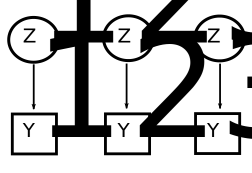
\includegraphics[scale=0.4]{Dag3.pdf}}}
\end{frame}

\begin{frame}[fragile]{Hidden Markov Chain simulation}
\begin{columns}
\begin{column}{0.5\textwidth}
\begin{knitrout}\tiny
\definecolor{shadecolor}{rgb}{0.969, 0.969, 0.969}\color{fgcolor}\begin{kframe}
\begin{alltt}
\hlcom{### observation simulation}
\hlstd{mu} \hlkwb{<-} \hlkwd{c}\hlstd{(}\hlnum{3}\hlstd{,} \hlnum{7}\hlstd{)}
\hlstd{sigma} \hlkwb{<-} \hlkwd{c}\hlstd{(}\hlnum{2}\hlstd{,}\hlnum{3}\hlstd{)}
\hlstd{Y.hmm} \hlkwb{<-} \hlkwd{rnorm}\hlstd{(N,} \hlkwc{mean}\hlstd{=mu[Z],} \hlkwc{sd}\hlstd{=sigma[Z])}
\hlkwd{plot}\hlstd{(Y.hmm,} \hlkwc{pch}\hlstd{=}\hlnum{19}\hlstd{)}
\hlkwd{plot}\hlstd{(Y.hmm,} \hlkwc{pch}\hlstd{=}\hlnum{19}\hlstd{,} \hlkwc{col}\hlstd{=Z}\hlopt{+}\hlnum{1}\hlstd{)}
\end{alltt}
\end{kframe}
\end{knitrout}
\end{column}
\begin{column}{0.4\textwidth}
\only<2>{\includegraphics[scale=0.3]{hmmCode2-1.pdf}}
\only<3->{\includegraphics[scale=0.3]{hmmCode2-2.pdf}}
\end{column}
\end{columns}
\end{frame}

\begin{frame}[fragile]{Sojourn time properties}


 {\small
  $T_i$, the sojourn time in State i follows a geometric distribution
 $$\P(T_i=l)=(\Pi_{ii})^{l-1}(1-\Pi_{ii})$$
 }


\begin{columns}
\begin{column}{0.5\textwidth}
\begin{knitrout}\tiny
\definecolor{shadecolor}{rgb}{0.969, 0.969, 0.969}\color{fgcolor}\begin{kframe}
\begin{alltt}
\hlstd{switchTime} \hlkwb{<-} \hlkwd{which}\hlstd{(}\hlkwd{diff}\hlstd{(Z)}\hlopt{!=}\hlnum{0}\hlstd{)}
\hlstd{sojournTime} \hlkwb{<-} \hlkwd{diff}\hlstd{(switchTime)}
\hlstd{sojournState} \hlkwb{<-} \hlkwd{rep}\hlstd{(}\hlkwd{c}\hlstd{(}\hlnum{3}\hlopt{-}\hlstd{Z[}\hlnum{1}\hlstd{], Z[}\hlnum{1}\hlstd{]),}
                    \hlkwc{length.out} \hlstd{=} \hlkwd{length}\hlstd{(sojournTime))}
\hlstd{br} \hlkwb{<-} \hlkwd{unique}\hlstd{(}\hlkwd{quantile}\hlstd{(sojournTime,}
                      \hlstd{p}\hlkwb{<-} \hlkwd{seq}\hlstd{(}\hlnum{1}\hlopt{/}\hlstd{N,} \hlnum{1}\hlstd{,} \hlkwc{length.out} \hlstd{=} \hlnum{6}\hlstd{)))}

\hlstd{abc} \hlkwb{<-} \hlkwd{seq}\hlstd{(}\hlnum{1}\hlstd{,} \hlkwd{max}\hlstd{(sojournTime)}\hlopt{+}\hlnum{10}\hlstd{)}
\hlkwd{lapply}\hlstd{(}\hlnum{1}\hlopt{:}\hlnum{2}\hlstd{,} \hlkwa{function}\hlstd{(}\hlkwc{i}\hlstd{)\{}
  \hlstd{var} \hlkwb{<-} \hlstd{sojournTime[sojournState}\hlopt{==}\hlstd{i]}
  \hlstd{br} \hlkwb{<-} \hlkwd{sort}\hlstd{(}\hlkwd{unique}\hlstd{(var))}
  \hlkwd{hist}\hlstd{(var,} \hlkwc{col}\hlstd{=i}\hlopt{+}\hlnum{1}\hlstd{,} \hlkwc{freq}\hlstd{=F,}
       \hlkwc{xlim}\hlstd{=}\hlkwd{range}\hlstd{(sojournTime),}
       \hlkwc{ylim}\hlstd{=}\hlkwd{c}\hlstd{(}\hlnum{0}\hlstd{,}\hlnum{0.4}\hlstd{),}
       \hlkwc{main}\hlstd{=}\hlkwd{paste0}\hlstd{(}\hlstr{"Sojourn Time, State "}\hlstd{, i),}
       \hlkwc{breaks}\hlstd{=br)}
  \hlkwd{lines}\hlstd{(abc,} \hlkwd{dgeom}\hlstd{(abc}\hlopt{-}\hlnum{1}\hlstd{,} \hlkwc{prob} \hlstd{=} \hlnum{1}\hlopt{-}\hlstd{PI[i,i]),}
        \hlkwc{col}\hlstd{=}\hlnum{1}\hlstd{,} \hlkwc{lwd}\hlstd{=}\hlnum{2}\hlstd{,} \hlkwc{lty} \hlstd{=} \hlnum{1}\hlopt{+}\hlstd{i)}
\hlstd{\})}
\end{alltt}
\end{kframe}
\end{knitrout}
\end{column}
\begin{column}{0.4\textwidth}
\only<2->{\includegraphics[scale=0.25]{hmmCode3-2.pdf}}\\
\only<3->{\includegraphics[scale=0.25]{hmmCode3-3.pdf}}
\only<4->{ see Semi Hidden Markov Model for removing this assumption}
\end{column}
\end{columns}
\end{frame}

\subsection*{Parameter estimation}
%%-----------------------------------------------------------------%%
%%-----------------------------------------------------------------%%


\begin{frame}{Statistical inference of incomplete data models} 
 \paragraph{Maximum likelihood estimate:} We are looking for
  $$
  (\widehat{\gammabf},\widehat{\Pibf}, \widehat{\nubf}) = \arg\max_{\gammabf, \Pibf, {\nubf}} \log P(\Ybf; \gammabf, \Pibf, \nubf)
$$
\only<1>{
    \begin{eqnarray*}
     \log P(\Ybf, \Zbf; \thetabf) & = & \hid{\sum_k Z_{1k} \log \nu_k }\\
     & &\hid{+ \sum_{i > 1} \sum_{k, \ell}
       Z_{i-1,k}Z_{i,\ell} \log \pi_{k\ell}} \\
     & & + \obsy{\sum_i \sum_k Z_{ik} \log f(y_i ; \gamma_k)} 
  \end{eqnarray*}
}
\only<2>{
  \begin{eqnarray*}
    \Esp\left( \log P(\Ybf, \Zbf)\vert Y_{1:N}\right)  & = & \Ehid{\sum_k\Esp\left( Z_{1k} \vert Y_{1:N}\right) \log \nu_k }\\
     & &\Ehid{+ \sum_{i > 1} \sum_{k, \ell}
      \Esp\left( Z_{i-1,k}Z_{i,\ell}\vert Y_{1:N}\right) \log \pi_{k\ell}} \\
     & & + \Eobsy{\sum_i \sum_k \Esp\left(Z_{ik}\vert Y_{1:N}\right) \log f(X_i ; \gamma_k)} 
  \end{eqnarray*}
}
\only<3>{
  \begin{eqnarray*}
   \Esp\left(  \log P(\Ybf, \Zbf) \vert Y_{1:N}\right) & = & \Ehid{\sum_k\P\left( Z_{1}=k \vert Y_{1:N}\right) \log \nu_k }\\
     & &\Ehid{+ \sum_{i > 1} \sum_{k, \ell}
      \P\left( Z_{i-1}=k, Z_{i}=l\vert Y_{1:N}\right) \log \pi_{k\ell}} \\
    & & + \Eobsy{\sum_i \sum_k \P \left( Z_{i}=k\vert Y_{1:N}\right) 
    \log f(X_i ; \gamma_k)}
  \end{eqnarray*}
}
\end{frame}

 
\frame{ \frametitle{EM Algorithm (Baum Welch)}
  \begin{itemize}
  \item Initialisation of $\thetabf^{(0)}=(\Pi, \gamma_1, ..., \gamma_K)^{(0)}$.
  \item While the convergence is not reached 
  \end{itemize}   
 \begin{description}
    \item[E-step] 
    \only<1>{Calculation of 
      \begin{eqnarray*}
        \tau^{(\ell)}_{ik}&=&P(Z_i = k | \Ybf, \thetabf^{(\ell-1)})\\
        \eta_{ikh}^{(\ell)} &=& \Esp[Z_{i-1,k}Z_{ih}| \Ybf, \thetabf^{(\ell-1)}]\\
      \end{eqnarray*}  }
     \only<2>{ Smart algorithm Forward-Backward algorithm  }
      
    \item[M-step] Maximization in $\thetabf=(\pibf, \gammabf)$ of
    \end{description} 
 $$
 \sum_k \tau^{(\ell)}_{1k}\log \nu_k
 + \sum_{i > 1} \sum_{k, h} \eta_{ikh}^{(\ell)} \log \pi_{kh}
 + \sum_i \sum_k \tau^{(\ell)}_{ik} \log f(y_i; \gamma_k) 
 $$
 }
\begin{frame}{Reconstruction of hidden state $\Zbf$}
\paragraph{Most credible value for $Z_i$:}
We are interested in 
$$\argmax_{k}\P(Z_i= k \vert \Ybf)=\argmax_k \tau_{ik}.$$
\pause
  \paragraph{Most credible sequence for $\Zbf$}
We are interested in 
$$\argmax_{k_1, \ldots k_n}\P(Z_1= k_1, \ldots Z_n=k_n \vert \Ybf)= ???$$
\pause
But force brut algorithm is not possible 
$$\longrightarrow \mbox{a smart algorithm : Viterbi algorithm}$$
\end{frame}


\begin{frame}{Viterbi algorithm}
\onslide<1->{\only<1>{
\paragraph{Key quantity:} The probability of the best hidden path from time 1 to $i$ who finished in $k$} 
\only<2->{
\paragraph{Key quantity:}
$$\delta_i(k)=\max_{k_1, \ldots k_{i-1}}\P(Y_{1:i}, Z_1=k_1, \ldots , Z_{i-1}=k_{i-1}, Z_i=k )$$ 
} 
}

\onslide<3->{
  \begin{itemize}
    \item \emph{Initialisation}
    \begin{eqnarray*}
      \delta_1(k) & = &\P(Z_1=k, Y_1) = \P(Z_1=k)
      \P(Y_1\vert Z_1=k)  = \nu(k) f_{\gamma_k}(y_1)\\
      \psi_1(k)& = &0
    \end{eqnarray*}
    \end{itemize}
}
\onslide<4->{
  \begin{itemize}
  \item \emph{Recurrence, for $i=1, \ldots n-1$}
  \begin{eqnarray*}
  \delta_{i+1}(k) & =& \max_{k_1,\ldots, k_i}
  \P(Y_{1:i}, Z_1=k_1, \ldots , Z_{i-1}=k_{i-1}, Z_i=k_i, Z_{i+1}=k )\\
  & =& \max_{k_i} \left\lbrace \delta_{i}(k_i) \P(Y_i\vert Z_{i}=k_i)\P(Z_{i+1}\vert   Z_{i}=k_i)\right\rbrace \\
\psi_{i+1}(k) & =&\argmax_{j}\left\lbrace \delta_i{j} \Pi_{jk}\right\rbrace
\end{eqnarray*}
\end{itemize}
}
\end{frame}

\begin{frame}[fragile]{Estimation of HMM with R}
\begin{knitrout}\tiny
\definecolor{shadecolor}{rgb}{0.969, 0.969, 0.969}\color{fgcolor}\begin{kframe}
\begin{alltt}
\hlkwd{library}\hlstd{(}\hlstr{'depmixS4'}\hlstd{)}

\hlstd{df} \hlkwb{<-} \hlkwd{data.frame}\hlstd{(}\hlkwc{Y}\hlstd{=Y)}
\hlstd{K}\hlkwb{=}\hlnum{2}
\hlstd{m1} \hlkwb{<-} \hlkwd{depmix}\hlstd{(Y}\hlopt{~}\hlnum{1}\hlstd{,}\hlkwc{data}\hlstd{=df,} \hlkwc{nstates}\hlstd{=}\hlnum{2}\hlstd{,} \hlkwc{family}\hlstd{=}\hlkwd{gaussian}\hlstd{())}
\hlstd{fit.model} \hlkwb{<-} \hlkwd{fit}\hlstd{(m1)}
\hlkwd{summary}\hlstd{(fit.model)}
\hlstd{Z.hat} \hlkwb{<-} \hlkwd{viterbi}\hlstd{(fit.model)[,}\hlnum{1}\hlstd{]}
\hlkwd{table}\hlstd{(Z, Z.hat)}
\end{alltt}
\end{kframe}
\end{knitrout}

\end{frame}


\begin{frame}{State Space model}
This is the trendy name for HMM, with potentially continuous value for $\Zbf$.

\pause
\begin{itemize}
\item $\Zbf$ is a sequence of hidden states and the observations $\Ybf$ are ruled by this sequence.
\begin{columns}
 \begin{column}{0.3\textwidth}
{\centering{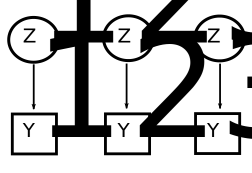
\includegraphics[scale=0.4]{Dag3.pdf}}}
\end{column}
\begin{column}{0.7\textwidth}
$\Zbf$ could be thougth as the actual locations and $\Ybf$ the observed locations.
\end{column}
\end{columns}

\pause
\item 
Estimation tools are EM algorithm or Bayesian framework (with monte carlo based estimation technics)
\end{itemize}
\end{frame}

% %--------------------------------------------------------------------
% %--------------------------------------------------------------------
\section{Late thoughts}
\begin{frame}{And more ...}
\begin{itemize}
\item It is possible to include dependency in $\Ybf$.
\item Markovian property could be removed (SHMM)
\item Presented methods may be used on several signals (ex $Speed$ and $angle$)
\item Work in progress for continuous time Markov model and dependent observations.
\end{itemize}
\blue{But}

\end{frame}

\begin{frame}{Limitations}
Trajectories are in continuous space and continuous time.
\begin{itemize}
\item Mostly, discrete time : effects of the sampling step and assumption of regularity.
\item Segmentation methods consider a signal in time,
\item Spatial information is lost.
\item Those methods are useful to identify different regimes of movement. This difference may be due to behaviour or the environment or interaction. 
\end{itemize}
\end{frame}

\begin{frame}
Many thanks to Emilie Lebarbier, Marie-Laure Martin-Magniette, Stéphane Robin for some contents of the slides.


\vspace{1cm}
Many thanks to Andrea and Linda for the invitation and organisation.

\end{frame}
\appendix
% \section{Probability Distribution for angles}
% 
% \frame{\frametitle{Circular Distribution}
% If $Z\sim WC(\mu,\gamma)$, $$f_{WC}(\theta;\mu,\gamma)=\sum_{n=-\infty}^\infty \frac{\gamma}{\pi(\gamma^2+(\theta-\mu+2\pi n)^2)}$$
% }

\end{document}
% %--------------------------------------------------------------------
% %--------------------------------------------------------------------

% %--------------------------------------------------------------------
% \frame{\frametitle{}
%   }


%   \vspace{-0.5cm}
%   \begin{tabular}{cc}
%     \hspace{-0.5cm}
%     \begin{tabular}{p{.5\textwidth}}
%     \end{tabular}
%     &
%     \hspace{-1cm}
%     \begin{tabular}{p{.5\textwidth}}
%     \end{tabular}
%   \end{tabular}
